\chapter{Research Results}
\begin{multicols}{2}
      \section{Research Topic}
      In research, it is paramount to have the formulation of a clear research topic, research main question,
      and research sub-questions. The main question serves as the focal point around which the research revolves,
      encapsulating the primary objective or purpose of the study.
      The following main research question will be used throughout the research:
      \begin{center}
            \textit{"How can Quality ICT B.V. effectively enhance API monitoring within its internal application
                  while integrating and leveraging SentinelOne EDR platform for continuous
                  cybersecurity monitoring while still ensuring adherence to the highest security standards?"}
      \end{center}
      The research sub-questions are then used to function as a pathway that dissects the main
      question into smaller, more manageable components, which can then be addressed individually. This approach
      allows for a more comprehensive and in-depth analysis of the research topic, ensuring that all relevant
      aspects are covered and that the research is conducted in a systematic and organized manner.
      This research main question is therefore expanded in the following research sub-questions: % data is not up to date, stop/pause the connection
      \begin{itemize}
            \item What is the current situation of the \acrshort{qaas} app of \acrlong{qict} \acrshort{bv}?
            \item What functionalities should be prioritized in the development of monitoring and managing
                  third-party \acrshort{api}s within the \acrshort{qaas} app while ensuring real-time monitoring,
                  error detection, and insight generation regarding \acrshort{api} connections?
            \item How can SentinelOne be integrated into the \acrshort{qaas} app environment, especially
                  aligning with the \acrshort{api} monitoring functionality, while still utilizing their key
                  features and capabilities in context of cyber-threat detection and remote \acrshort{it}
                  infrastructure management?
            \item What are the most suitable visualization techniques for displaying the data processed and
                  received by the \acrshort{qaas} app in \acrshort{xml} and \acrshort{json} formats to ensure
                  clear and insightful representation of threats detected by SentinelOne \acrshort{api}?
      \end{itemize}
      \section{Research Methodology}
      In this research, different research methods have been used to answer the research questions. This research
      will be based on the six \acrshort{ict} research methods defined by HBO-I (\cite{ictresearchmethods}). A
      research method for each sub-question is then defined along with how the results are considered valid and
      reliable:
      \subsection{Method of Data Collection}
      \begin{itemize}[label=-]
            \item Sub-question \#1: desk research of Literature Study will be conducted, with the goal of creating
                  infrastructure information that displays the structure of the \acrshort{qaas} app and all of its
                  dependencies. Furthermore, Interview with key stakeholders involved in the  development, maintenance,
                  and usage of the \acrshort{qaas} app will be conducted to gain insights into the current situation
                  of the app.
            \item Sub-question \#2: Literature Study on various articles on the Internet, interviews, expert reviews,
                  and requirement elicitation techniques such as use case analysis and user stories. Analysis on the
                  current \acrshort{qaas} app and its \acrshort{api} monitoring capabilities.
            \item Sub-question \#3: technical evaluations of SentinelOne's capabilities and \acrshort{api}s will
                  be conducted, the \acrshort{api} documentation and integration guideline will be read and review
                  with Literature Study method and case studies of similar integrations. Requirements from the
                  cybersecurity experts from the \acrshort{qict} department responsible for SentinelOne's technical
                  support will be gathered and analyzed. Furthermore, Prototyping with proof-of-concept prototypes
                  on a test environment will be conducted to test different integration scenarios, assess feasibility,
                  identify potential challenges, refine the approach, and evaluate the performance of the integration.
            \item Sub-question \#4: research into existing visualization techniques for \acrshort{xml} and
                  \acrshort{json} data, especially the data coming from SentinelOne \acrshort{api} through Literature
                  Study. Analyze existing data visualization tools and platforms that are available in Flutter and
                  Firebase. Gather requirements from project stakeholders regarding data visualization preferences and
                  usability, and do data analysis and usability testing.
      \end{itemize}
      \subsection{Selected Measuring Instruments}
      \begin{itemize}[label=-]
            \item Sub-question \#1: structured interview guide, document report checklist analysis and review,
                  observation, analysis tools for codebase and logs, and quite possibly supplemented by surveys
                  or questionnaires.
            \item Sub-question \#2: document analysis tools for literature review. Structured questionnaires for
                  requirement interviews regarding functionality rating scale and compare the response against
                  industry standards and best practices. Observation of existing \acrshort{api} monitoring tools.
                  Prioritize functionalities based on importance, feasibility, and impact on the \acrshort{qaas} app.
            \item Sub-question \#3: technical assessments and requirement workshops will be conducted. Furthermore,
                  \acrshort{api} documentation  review, document analysis tools, security impact risk assessment,
                  and feasibility checklist assessment with the Company Supervisor will also be overseen.
            \item Sub-question \#4: the selected measuring instruments for this sub-question will be through
                  observation of existing data visualization tools, literature review through reading the studies of
                  the best visualization suitability matrix techniques, structured questionnaires to end-user
                  interviews, and usability testing heuristics.
      \end{itemize}
      \subsection{Method of Data Analysis}
      \begin{itemize}[label=-]
            \item Sub-question \#1: a qualitative thematic \acrshort{swot} analysis of interview transcripts
                  and documentation for operational insights to identify strengths, weaknesses, and areas for
                  improvement in the current situation of the \acrshort{qaas} app.
            \item Sub-question \#2: comparative analyze survey/interview responses using \acrshort{mcda} and
                  compare against industry standards and best practices. Prioritize functionalities based on
                  importance, feasibility, and impact on the \acrshort{qaas} app.
            \item Sub-question \#3: evaluate the technical feasibility, compactibility, and alignment of
                  SentinelOne's features with the \acrshort{qaas} app environment. Analyze potential integration
                  challenges and mitigation strategies, and assess the performance of the integration through
                  prototyping and testing. Technical analysis for the \acrshort{api} documentation and
                  thematic analysis for interview data.
            \item Sub-question \#4: technical tool analysis by reviewing and evaluating the suitability of different
                  visualization techniques for representing the data processed and received by the \acrshort{qaas}
                  app in \acrshort{xml} and \acrshort{json} formats from the \acrshort{api} considering factors such
                  as clarity, interpretability, and user engagement. Do a user-centered design and cognitive load
                  analysis by analyzing feedback from company stakeholders, supervisor, and end-users.
      \end{itemize}
      \subsection{Reliability, Validity, and General Applicability}
      \begin{itemize}[label=-]
            \item Sub-question \#1: the reliability of the data can be ensured by triangulation of data from
                  multiple sources and conducting interviews with stakeholders from different departments with
                  structure questionnaires to ensure that the data is consistent and accurate. The validity of
                  the data will be ensured by  cross-referencing with the existing literature or industry best
                  practices or other sources and  through information obtained from  interviews with the
                  \acrshort{qaas} app developers to ensure  that the data is accurate and reliable. The general
                  applicability of the data will be ensured by  ensuring that the information obtained is relevant
                  and applicable to the research question and  that it can be used to draw meaningful conclusions
                  and make informed decisions, furthermore by comparing findings with industry standards and best
                  practices or similar case studies or projects.
            \item Sub-question \#2: ensure reliability through sampling techniques and representative stakeholder
                  involvement, with comprehensive literature review and multiple sources of information. Validate
                  priorities against real-world scenarios or case studies involving diverse expert panel, like
                  the Company Supervisor. General applicability can be assessed by comparing prioritization with
                  similar projects or frameworks, and considering scalability and adaptability of the integration
                  with representative user samples.
            \item Sub-question \#3: the validity of this sub-question will be through pilot integration unit testing
                  or proof of concept documents, and ensuring alignment with cybersecurity standards and best
                  practices. The reliability will be to consider future needs such as adaptability and scalability of
                  the integration, and focus on \acrshort{qict} user context and needs. General applicability can be
                  assessed by comparing integration strategies with industry standards or expert opinions such as from
                  the Company Supervisor.
            \item Sub-question \#4: reliability can be defined by ensuring future adaptability with comprehensive
                  literature review and multiple sources of information. Validity can be achieved through validating
                  visualization choices through data-driven approach in usability testing or  prototyping, ensuring
                  alignment with best practices in data visualization and involving the expert, like the Company
                  Supervisor on the field. General applicability can be assessed by accessibility considerations by
                  comparing proposed visualization techniques with similar applications or domains.
      \end{itemize}
      \subsection{Research Limitations}
      The project and research in general will be limited on the \acrshort{api} request methods, in which the author
      is allowed to do only GET requests. This is due to the fact that the author is not allowed to do any PATCH,
      POST, PUT, DELETE, or any other \acrshort{http} request methods that could potentially change the state of the
      \acrshort{qaas} app or the \acrshort{api} that is being requested. This limitation is because the author is not a
      full-time employee of \acrshort{qict} and is not allowed to make any changes to the \acrshort{qaas} app or the
      \acrshort{api} that is being requested. Therefore, the author is limited to do research in the best practices
      and possible answer for \acrshort{api} monitoring and integration for the GET request method only.

      Moreover, the author is also limited to the non-disclosure agreement signed within the initialization period of
      the graduation work placement. This means that any confidential information that the company deems as confidential
      will not be disclosed in this research. This includes any information that is not publicly available, such as any
      financial data or security data pertaining to the internal system or the \acrshort{qaas} app internal code.
      \section{Research Sub-Question \#1}
      The \acrshort{qaas} app is an \acrshort{erp} web application that is used by \acrshort{qict} and its clients.
      For \acrshort{qict}'s clients, it is a \acrshort{saas} that is used.... For \acrshort{qict} itself, it is an
      \acrshort{erp} system that is used to manage the clients and their \acrshort{ict} infrastructure.
      It is made in Dart with Flutter as the front-end framework. There are 2 main parts of the \acrshort{qaas} app, the
      front-end and the back-end. The front-end is made in Flutter, and the back-end is made in Node.js with TypeScript
      as the template. The back-end is hosted on Firebase Cloud Functions which are used to connect and make
      \acrshort{http} calls to the internal \acrshort{api}s, and the front-end is hosted on Firebase Hosting.

      \subsection{QaaS App Infrastructure}
      \subsubsection{Flutter}
      Flutter is an open-source framework made by Google in 2017. It used as an \acrshort{ui} toolkit for building
      natively compiled applications for mobile, web, and desktop (Windows, mac\acrshort{os}, Linux) from a single
      codebase (\cite{flutter}).

      \subsubsection{Cloud Solutions}
      \subsubsection{Firebase}
      Firebase is a comprehensive platform for developing and managing web and mobile applications, created by
      Google and is party of \acrshort{gcp}. It was originally an independent company founded by Firebase, Inc.
      in 2011. It was then acquired by Google in 2014. Since then, it has become an integral part of Google's
      broader ecosystem of cloud services (\cite{firebase}).

      Firebase is a \acrshort{baas} that provides developers with a variety of tools and services to help with both
      back-end infrastructure and front-end capabilities without worrying about managing servers or infrastructures.
      The services offered by Firebase including (\cite{firebaseproducts})
      \begin{itemize}
            \item Databases:
                  \begin{itemize}
                        \item Firestore Database: Firestore is a \acrshort{nosql} database that is part of the Firebase
                              platform. It is a flexible, scalable database for mobile, web, and server development. It keeps
                              data in sync across client apps through real-time listeners and offers offline support for mobile
                              and web, so the developers can build responsive apps that work regardless of network latency or
                              Internet connectivity.
                        \item Real-time database:
                  \end{itemize}
            \item Authentication: is an easy-to-understand authentication services that support various authentication
                  methods like email/password, phone number, with identity providers such as Google, Facebook, Twitter,
                  Apple, GitHub, \acrshort{etc}
                  along with utilizing \acrshort{2fa} authentication factors to enhance security by requiring additional
                  factor, such as an \acrshort{otp} code that is sent to the user's phone or security key.
            \item Cloud Functions: often just called Functions in the Firebase console, it allows developers to run
                  back-end code in response to events triggered by Firebase features and \acrshort{https} requests.
                  The code is stored in Google's cloud and runs in a managed environment. It is a serverless framework
                  that allows developers to build and deploy serverless functions that automatically scale up and down
                  based on demand. The available programming languages are Node.js (\acrshort{js} and \acrshort{ts}),
                  Python, Go, Java, and .NET (C\#). Cloud Functions offers 2 product versions: the original version
                  (1st gen), and the 2nd gen which is built on Cloud Run and Eventarc to provide an enhanced feature set.
                  \begin{itemize}
                        \item 1st Generation: Most of the Firebase Cloud Functions that are used in the \acrshort{qaas} app
                              are in this version. The company wishes to migrate all the functions to the 2nd generation in
                              the future.
                        \item 2nd Generation: The company wishes that the author's graduation project will utilize the 2nd
                              generation of Cloud Functions. Features in the 2nd generation including:
                              \begin{itemize}
                                    \item Longer request processing times
                                    \item Larger instance sizes
                                    \item Traffic management
                                    \item Eventarc integration
                                    \item Broader CloudEvents support
                              \end{itemize}
                  \end{itemize}
      \end{itemize}
\end{multicols}

\begin{longtable}{|p{5cm}|p{5.5cm}|p{5.5cm}|}
      \hline
      \rowcolor{blue!20}
      Feature         & 1st Gen                                                     & 2nd Gen                                                       \\
      \endfirsthead
      \hline
      Image registry  & Container Registry or Artifact Registry                     & Artifact Registry only                                        \\
      \hline
      Request timeout & Up to 9 minutes                                             & \begin{itemize}
                                                                                            \item Up to 60 minutes for \acrshort{http}-triggered functions
                                                                                            \item Up to 9 minutes for event-triggered functions
                                                                                      \end{itemize} \\
      \hline
      Instance Size   & Up to 8\acrshort{gb} \acrshort{ram} with 2 v\acrshort{vcpu} & Up to 16\acrshort{gb} \acrshort{ram} with 4 \acrshort{vcpu}   \\
      \hline
      Concurrency     & 1 concurrent request per functions instance                 & Up to 1000 concurrent requests per function instance          \\
      \hline
      \caption{Comparison between the 1st and 2nd Generation of Cloud Functions}
      \label{tab:restvsoap}
\end{longtable}

\begin{multicols}{2}
      \begin{itemize}
            \item Hosting: a service that allows developers to host static websites, dynamic web apps, mobile apps, and
                  microservices on Firebase's infrastructure. The \acrshort{qaas} app is currently hosted on Firebase
                  Hosting.
            \item Cloud Messaging/\acrshort{fcm}: allows developers to send push notification and targeted messages to a
                  client app that new email or other data is available to sync, or send notification messages to drive app
                  interaction, adding more user re-engagement and retention. It is a cross-platform messaging solution that lets
                  developers reliably deliver messages at no cost.
            \item Cloud Storage: offers a secure, scalable, and reliable file storage and sharing for Firebase apps.
                  It is designed to help developers quickly and easily store and serve user-generated content, such as
                  photos or videos.
            \item Remote Config: allows developers to dynamically control and the change behaviour and appearance of their apps
                  without publishing app updates and requiring users to download them.
            \item Performance Monitoring
            \item Analytics: provides free and unlimited analytics solutions for understanding app usage, user engagement and
                  user behaviour by tracking event logging, user demographics, and funnel analysis to gain valuable insights to
                  improve the app.
            \item Crashlytics: is a lightweight, real-time crash and error reporter that helps developers track, prioritize,
                  and fix stability issues that erode to the quality of the developer's app.
            \item Test Lab: enables automated testing of the developer's app on real devices in the Google data center.
            \item Dynamic Links: consist of deep links that dynamically route users to the content they are interested in,
                  across platforms and devices. It helps developers create and share links that work the way they want, on the
                  platform they want, and whether users have their apps installed.
            \item \acrshort{ml} Kit: provides a set of \acrshort{ml} \acrshort{api}s that can be easily integrated developer's app.
                  This feature is still in beta testing.
      \end{itemize}

      \textbf{JavaScript}

      \acrshort{js} is a high-level, interpreted programming language that conforms to the \acrshort{ecma}Script specification.
      It is a multi-paradigm programming language, supporting \acrshort{oop}, imperative, and functional programming styles and
      is primarily used for client-side web development. It is also used for server-side development with Node.js, and for
      mobile app development with frameworks like React Native, Vue.js, Angular.js, and NativeScript. \acrshort{js} is now one
      of the core technologies of the web, along with \acrshort{html} and \acrshort{css}, and is supported by all modern web
      browsers. Some key features of \acrshort{js} include:
      \begin{itemize}
            \item Client-side Scripting: it is mainly used for client-side scripting in web browsers, allowing programmers to
                  create dynamic content that interacts with the browser and the user. It can manipulate the content and behavior
                  of \acrshort{html} elements, respond to user actions without the need to reload the page for interacting with
                  \acrshort{dom} to update page content dynamically. This enhances the \acrshort{ux} by making web applicaitons
                  feel more responsive and integrated.
            \item Cross-Platform Compactibility: it is supported by all modern web browsers, including Chrome, Firefox, Safari,
                  Opera, and Edge, and can be used to build cross-platform web applications that run on any device or platform,
                  like Android or i\acrshort{os}.
            \item Server-Side Scripting: with the advent of Node.js, it has also become popular for server-side scripting. Node.js
                  is a runtime environment that allows developers to build scalable network applications, including web servers,
                  \acrshort{api}s, and real-time applications like chat servers. This has expanded the versatility and use cases of
                  \acrshort{js} beyond the browsers, making it a full-stack development language.
            \item Dynamic Typing: it means that variables do not have predetermined types. Instead, types are determined at runtime
                  based on the assigned values.
            \item Functional Programming: it supports concepts such as first-class functions, high-order functions, and closures.
                  This allows programmers to write more concise and expressive code by treating functions as first-class citizens.
            \item Event-Driven Programming: it follows an event-driven programming paradigm, where actions or events trigger specific
                  functions or code execution, makes it well-suited for building interactive \acrshort{ui} and handling user interaction.
      \end{itemize}
      \textbf{Node.js}

      is an open-source, cross-platform, server-side runtime environment built on Chrome's V8 \acrshort{js} engine that allows
      programmers to run \acrshort{js} code outside a web browser, enabling the development of server-side and networking applications.

      \textbf{TypeScript}

      is an open-source programming language developed and maintained by Microsoft. It is a superset of \acrshort{js}, meaning that any valid
      \acrshort{js} code is also valid in \acrshort{ts}. It adds optional static typing to \acrshort{js}, which allows developers to annotate
      their code with type information, catch errors early in the development, and improve the maintainability or large codebases. Some
      developers prefer using \acrshort{ts} over \acrshort{js} for some of its key-features:
      \begin{itemize}
            \item Static Typing: it checks the types of variables at compile-time, which enable developers to specify the types of variables,
                  functions parameters, and return values. This introduces type safety, in contrast to \acrshort{js} which is dynamically typed,
                  which means that the types of variables are determined at runtime.
            \item Enums: it provides supports for enums, allowing developers to define a set of named constants with associated values.
            \item Generics: it supports generics, enabling the creation of reusable components that can work with a variety of data types.
            \item Decorators: it supports decorators, which are a way to add annotations and a meta-programming syntax for class declarations
                  and  members. Decorators can be used to modify classes, methods, and properties at design time, providing a powerful way to
                  extend or modify the behaviour of classes and their members.
            \item Interfaces and Classes: it supports \acrshort{oop} concepts such as classes, interfaces, inheritance, and access modifiers,
                  making it easier to organize and structure code.
            \item \acrshort{es}6+ Features: it supports many features introduced in \acrshort{ecma}Script standards beyond \acrshort{es}5,
                  such as arrow functions, classes, async/await syntax, and modules.
            \item Backwards Compactibility: it is designed to be backwards compactible with \acrshort{js}, which means that developers can use
                  it alongside \acrshort{js} code and integrate it into existing \acrshort{js} projects and environments, including, browsers,
                  Node.js, and other \acrshort{js} runtime environments.
      \end{itemize}
\end{multicols}

\begin{figure}[htbp]
      \centering
      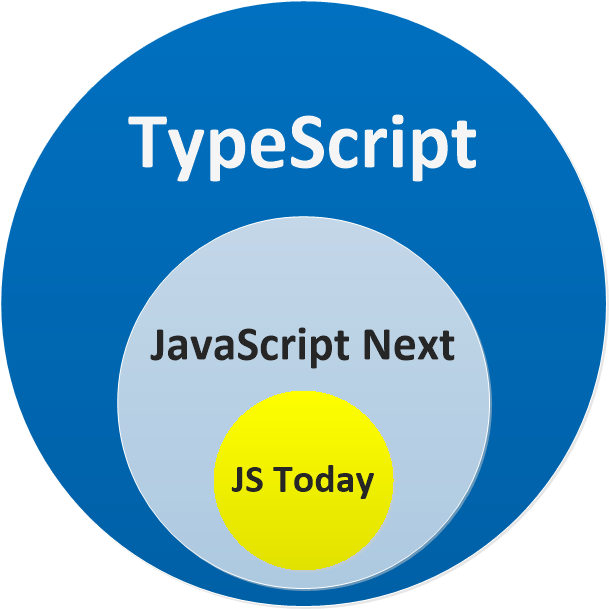
\includegraphics[width=0.6\textwidth]{Figures/TSJSVenn.png}
      \caption{Venn diagram of TypeScript and JavaScript}
      \label{fig:tsjsvenn}
\end{figure}

\begin{multicols}{2}

      \textbf{Algolia}

      Algolia is used for search functionality. It is a search-as-a-service platform that enables developers to
      integrate and build fast, relevant search functionality into their applications and websites (\cite{algolia}).
      It provides a range of features and capabilities for building and managing search functionality, including
      full-text search, typo tolerance, and relevance tuning, as well as analytics and monitoring tools to help
      developers understand how users are interacting with their search functionality in real-time.

      The reason as to why \acrshort{qict} uses Algolia is that the nature of Firebase search engine is quite often
      proven to be inaccurate and slow.

      \textbf{Secret Manager}

      It is a fully managed service provided by \acrshort{gcp} that allows developers and organization to securely store,
      access, and manage sensitive information such as API keys, passwords, certificates, \acrshort{oauth} credentials,
      \acrshort{db} credentials and other credentials used in throughout the lifecycle of their applications
      (\cite{googlesecretmanager}). It is not part of Firebase, and it helps the \acrshort{qaas} app to centralize and
      secure its secrets in scalable and easily manageable way. Key-features of Secret Manager include:
      \begin{itemize}
            \item Secure Storage: it encrypts the secret values using \acrshort{cmek}, ensuring the sensitive data is protected
                  both at rest and in transit.
            \item Audit Logs: it provides and manages audit logs that record all access and modification of activities, helping
                  developers meet compliance, better accountability and regulatory requirements.
            \item Versioning and Automatic Rotation: it supports versioning of secrets, allowing developers to store multiple versions
                  of the same secret. This means that the developers get to keep multiple versions of secrets and easily revert or roll
                  back to a previous version if needed, which will help in auditing and tracking changes to secrets over time. This feature
                  enables automatic seamless rotation of secrets at regular intervals without  disrupting the applications, which improves
                  the security part of the application by ensuring that secrets are regularly updated without manual intervention.
            \item Access Control: it provides fine-grained access control using Google \acrshort{iam}, allowing developers to specify
                  who can access and manage the stored secrets and what they can do with them.
            \item Centralized Management: it stores and manages all secrets in one place, simplifying access and control.
      \end{itemize}

      \textbf{NoSQL Database}

      is a category of \acrshort{db} that provides a mechanism for storage and retrieval of data that is modelled in ways other
      than the tabular relations used in \acrshort{rdbms}. \acrshort{nosql} \acrshort{db}s are typically designed to handle large
      volumes of unstructured or semi-structured data, such as \acrshort{json}, \acrshort{xml}, or binary objects, and they offer
      a flexible data model that can evolve over time. Both databases in Firebase, Firestore, and Real-time Database are \acrshort{nosql}
      databases. Some characteristics of \acrshort{nosql} \acrshort{db}s include (\cite{nosql}):
      \begin{itemize}
            \item Data Model: \acrshort{nosql} uses dynamic schema, which allows data to be inserted without having to define the schema
                  first, while \acrshort{sql} uses a fixed schema to store data.
            \item Data Structure: \acrshort{nosql} \acrshort{db}s use a variety of data structures such as key-value pairs, document-oriented,
                  graphs databases, and columns-oriented; unlike \acrshort{sql} which only uses tables to store data.
            \item Querying: \acrshort{nosql} uses variety of query languages, such as Mongo\acrshort{db} query language or Cassandra's
                  \acrshort{cql}, while \acrshort{sql} databases only use \acrshort{sql} as the unified language to query data.
            \item Data Consistency and \acrshort{acid} Compliance: databases that are \acrshort{acid} compliant means that they follow a
                  set of rules to ensure that database transactions are processed reliably and securely. \acrshort{sql} databases are a
                  good example of this, while \acrshort{nosql} databases sacrifice some \acrshort{acid} properties in order to achieve
                  higher performance and scalability.
            \item Use Case: \acrshort{nosql} \acrshort{db}s are ideal for applications that need to handle large volumes of data and
                  require high scalability and flexibility, such as social media platforms, real-time analytics, and content management
                  systems.
            \item Scalability: \acrshort{nosql} databases are traditionally designed for horizontal scalability, meaning they can easily
                  scale out multiple servers or clusters to handle volumes of data and high throughput, which is more cost-effective and
                  allows for better scalability. They are well-suited for distributed and cloud-based environments. \acrshort{sql} databases
                  are traditionally designed for vertical scalability, meaning a single server is scaled up with more powerful hardware and
                  power (\acrshort{cpu}, \acrshort{ram}) to a single server. This can become expensive and limit scalability.
      \end{itemize}
      "Serverless Architecture"
\end{multicols}

\begin{figure}[htbp]
      \centering
      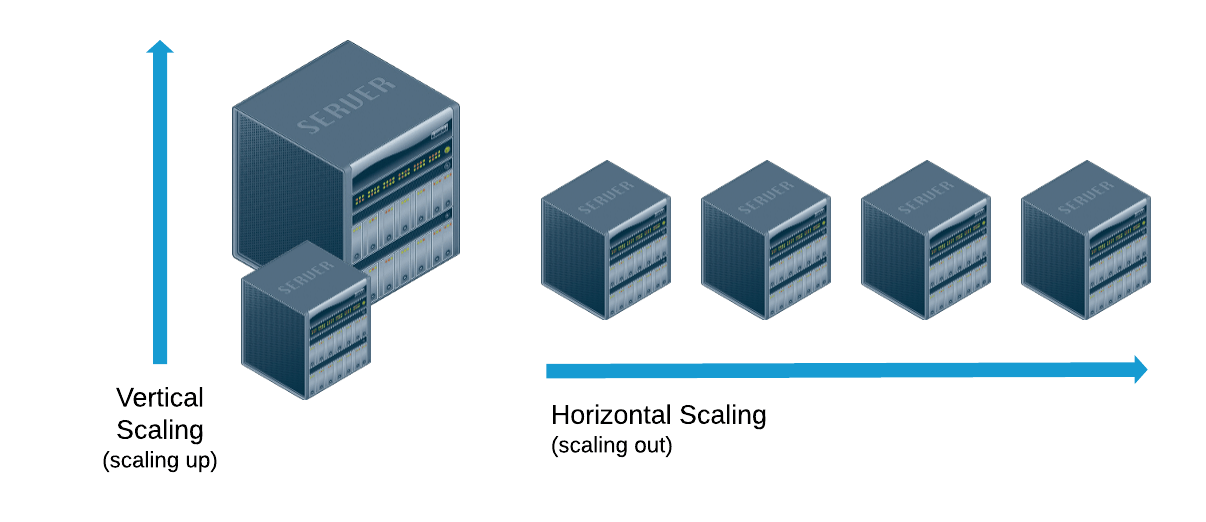
\includegraphics[width=0.8\textwidth]{Figures/nosql-scalling.png}
      \caption{Vertical (\acrshort{sql}) \acrshort{vs} Horizontal (\acrshort{nosql}) Scaling}
      \label{fig:graphqlvsrestarchitecture}
\end{figure}

\begin{multicols}{2}
      Some examples of \acrshort{nosql} databases include Mongo\acrshort{db} (document-oriented), Cassandra (wide-column store), Redis
      (key-value store), and Neo4j (graph database). Some examples of \acrshort{sql} databases include My\acrshort{sql},
      Postgres\acrshort{ql}, and \acrshort{ms} \acrshort{sql} Server.
      \subsection{Q-ICT Internal APIs}
      \subsubsection{What is an API?}
      \acrshort{api} is a software intermediary that allows two applications to talk to each other. They are an
      accessible way to extract and share data within and across organizations.
      \subsubsection{Web APIs}
      A web \acrshort{api} is an \acrshort{api} that can be accessed using the \acrshort{http} protocol. Not all
      \acrshort{api}s are web \acrshort{api}s; some \acrshort{api}s are used only to communicate between two
      applications on the same computer, never making use of a web connection. But in practice, when developers talk
      about \acrshort{api}s, they are almost always talking about web-based \acrshort{api}s used to

      \textbf{JSON format}
      \acrshort{json} is a lightweight data-interchange format that is easy for humans to read and write while being
      also easy for machines to parse and generate too. It is based on a subset of the JavaScript programming language
      and is commonly used for representing structured data. \acrshort{json} is often used for transmitting data between
      a server and a web application, as well as for storing configuration data.

      \acrshort{json} data is organized into key-value pairs, where keys are strings and value can be strings (enclosed
      in double quotes `""`), booleans (`true` or `false`), numbers, objects (unordered collections of key-value pairs
      enclosed in curly braces '{}'), arrays (ordered collections of values enclosed in square brackets '[]'), or null.
\end{multicols}

\begin{lstlisting}[language=JSON, caption=Example of a JSON response, label=lst:jsonresponse]
      {
            "name": "John Doe",
            "age": 30,
            "isStudent": false,
            "cars": [
                  { "name": "Ford", "models": ["Fiesta", "Focus", "Mustang"] },
                  { "name": "BMW", "models": ["320", "X3", "X5"] },
                  { "name": "Fiat", "models": ["500", "Panda"] }
            ],
            "hobbies": ["Reading", "Gaming", "Traveling", "Cooking", "Photography", "Painting", "Gardening"],
            "address": {
                  "street": "Sesame Main Street",
                  "city": "New York",
                  "zip": "10001"
            }
      }
\end{lstlisting}

\begin{multicols}{2}
      \textbf{XML format}
      \acrshort{xml} is a markup language that defines a set of rules for encoding documents in a format that
      is both human and machine-readable. It provides a way to structure data in a hierarchical format using
      tags to define elements and attributes within those elements. It is often used for store, design, and
      representing structured data in a portable and platform-independent way, making it easy to create,
      exchange, and process information between different systems, applications, and platforms.

      \acrshort{xml} documents consist of text-based data enclosed in tags, similar to \acrshort{html}, but
      allows users to define their own customized tags and document structures. This flexibility makes
      \acrshort{xml} suitable for representing a wide variety of data types and structures.

      \acrshort{xml} is often used in various domains such as web services, configuration files, data
      interchange between different software systems, and more.
\end{multicols}

\begin{lstlisting}[language=XML, caption=Example of a XML response, label=lst:xmlresponse]
      <?xml version="1.0" encoding="UTF-8"?>
      <response>
          <status>200</status>
          <message>OK</message>
          <data>
              <user>
                  <id>123</id>
                  <username>johndoe</username>
                  <email>johndoe@example.com</email>
                  <role>user</role>
              </user>
              <user>
                  <id>456</id>
                  <username>janedoe</username>
                  <email>janedoe@example.com</email>
                  <role>admin</role>
              </user>
          </data>
      </response>
\end{lstlisting}

\begin{multicols}{2}
      \textbf{OpenAPI Standard}
      Previously known as Swagger, \acrshort{oas} is a specification for writing a public \acrshort{api}, with
      guidelines for details like endpoint naming conventions, data formats, and error messaging
      (\cite{openapistandard}). The standards required by Open\acrshort{api} and its automation of some tasks
      make it easier for a developer to start working with an \acrshort{api} without needing to read through
      a complex code base. For \acrshort{api} producers, Open\acrshort{api} standard offers access to a wide
      variety of tools based on the standards. \acrshort{api} teams can use these tools to quickly up mock
      servers and create high-quality documentation, among other tasks.
      \acrshort{api}s are generally categorized into different types based on their audience, architecture, and
      protocols (\cite{typesofapi}):
      \subsubsection{Different Types of API By Audience}
      \textbf{Public API}: also called external or Open \acrshort{api}, and as the name suggests it is available
      to everyone. They are open for the public to use and integrate with their applications. Developers can quickly
      implement them using little to no authorization, with few require sign-up and generation of the \acrshort{api} Keys
      to access them. This can make them to not be the best regarding security - just because "public" means expanded
      visibility - but sharing data with them is easier.

      Examples of a public \acrshort{api} are OpenWeatherMap, Google Maps navigation, Facebook and the Twitter \acrshort{api},
      which the latter allows  developers to access Twitter's functionality and data.

      \textbf{Internal API}: also called Private \acrshort{api}, and is used within a private organization to make internal
      apps "talk" to each other. To interact with the data, a developer needs to be actively granted permission to access it,
      because the data and functionality available through the \acrshort{api} are proprietary to the company. They are often
      set up with extensive logging and load-balancing capabilities because they must have greater fault tolerance and
      security than public \acrshort{api}s. They also do not follow the Open\acrshort{api} standard as consistently
      as public \acrshort{api}s, since their producers and consumers typically work together closely, data formats
      can be negotiated based on specific use cases. As they are built by specifically the company; it will only have
      \acrshort{api} protocol types that the organization wants to support. All the \acrshort{api}s managed by the
      \acrshort{qaas} app fall into this category. This solution tend to be very secure, as they are entirely internal.

      \textbf{Partner API}: also called Shared \acrshort{api}, this \acrshort{api} is made considering the scalability
      while developing the business, which will share a few \acrshort{api}s across a few other licensed organizations,
      enabling service offerings across business (\acrshort{b2b}). This \acrshort{api} is shared only with the intended
      users; others might not have access to them because they are not shared publicly, thus making it exists somewhere
      between public and private \acrshort{api}s. They often function to share data between two companies or organizations
      for a specific business purpose, while still ensuring strict privacy protection.

      These \acrshort{api}s indeed require authorization to access them (like having a PayPal account or an \acrshort{api}
      key). All the clients who are part of the business can access and integrate using those \acrshort{api}s. Few
      \acrshort{api}s will only provide read access, and few will provide read/write access via shared \acrshort{api}s.
      This depends on the business process model.

      For example, travel booking \acrshort{api}s are shared with travel agencies to increase their visibility and
      booking. Websites like Expedia, Make My Trip, and Trivago are excellent examples of this kind of \acrshort{api}.

      \textbf{Composite API}: it connects multiple \acrshort{api}s into a single data or interface or process to
      streamline the development operations, therefore allowing developers to bundle and send requests from different
      \acrshort{api}s as they do not have to write separate code for every individual \acrshort{api}. Usually,
      one or more related \acrshort{api}s are combined to improve performance. They reduce the load to the server
      as they are treated as a single call. In the microservice-based architecture
      (\textit{\nameref{microservicesapi}}), a single user action might involve multiple calls, which can come as
      a drawback as they generate enormous number of individual \acrshort{api} calls. In that scenario, the orchestration
      of this type of \acrshort{api} is very helpful as this work faster and is easier to implement. It is more secure
      than using multiple, individualized solutions, and it may also support multiple \acrshort{api} protocol types.

      A good example of this type is Shopify \acrshort{api}, which provides synchronization to large volumes of data and
      actions with other platforms that are dependent on each other in one request, such as Etsy, eBay, and Amazon. Rather
      than having multiple \acrshort{api}s to manage the automation of inventory, shipping, and taxes across multiple shopfronts,
      a single \acrshort{api} can be used for syncing and integration. Similar in ordering via a food app, the customers can
      use multiple GET calls, retrieving the food, and finally placing the request as a POST call.
      \subsubsection{Different Types of API by Architecture}
      \textbf{Monolithic API}: this is a single, coherent codebase type of architecture, providing access to a complex data
      source. Most public \acrshort{api}s are monolithic \acrshort{api}s, because it is familiar to most web developers, and
      they often closely follow the \acrshort{mvc} architecture of a relational \acrshort{db}. They provide predictable
      functionality across a range of resources, and they generally remain fairly stable over time because they serve so
      many use cases for many users.

      However, as the name suggests, they are monolithic, and therefore can be difficult to scale or refactor, because so much
      data is interconnected with them. When developers worry about releasing "breaking changes", they are often working with
      monolithic architectures, where changing even minor details can have unpredictable consequences.

      \textbf{Microservices API} \label{microservicesapi}: this is the main alternative to monolithic \acrshort{api}
      architecture. This architecture is more common for internal and partner \acrshort{api}, though public \acrshort{api}
      may also be part of an organization's overall microservice architecture. Most development teams using a
      \acrshort{ci}/\acrshort{cd} process make use of many microservices as part of their code lifecycle, each serving a
      discrete, independent purpose. For example, an e-commerce company might have an internal microservice that
      provides inventory data, and another to validate employee geolocation on changes to inventory data, while
      software developers pushing code automatically call microservices for testing and governance. As workflows
      change, individual microservices can be swapped out, updated, or replaced without affecting the overall parts
      of the system.

      \textbf{Unified API}: this type is common among Partner \acrshort{api}s. It serves similar purpose to Composite
      \acrshort{api}s, but instead it bundles related calls to multiple different \acrshort{api}s, instead of to multiple
      endpoints on a single \acrshort{api}.

      \subsubsection{Different Types of API Protocols}\label{chap:typesofapis}
      \textbf{\acrshort{soap} \acrshort{api}s}: are strictly based on \acrshort{xml} for the message structure and
      \acrshort{http} for the protocols. \acrshort{soap} itself is a protocol and sending a \acrshort{soap}
      request is similar to using an envelope to send a message. \acrshort{soap} \acrshort{api}s consume extra
      overhead and more bandwidth, and require more work on both the client and server ends. That being said,
      like envelopes, \acrshort{soap} encloses more stringent security compared to \acrshort{rest}. \acrshort{xml}-encoded
      \acrshort{soap} messages use the format defined below:
      \begin{itemize}
            \item \textbf{Envelope}: the root element of the message, which encapsulates the entire
                  \acrshort{soap} message. It 'envelopes' the message by placing tags at the start and the end.
            \item \textbf{Header (optional)}: defines specific additional message requirements, such as authentication.
            \item \textbf{Body}: the request of response is included here.
            \item \textbf{Fault (optional)}: information about errors that might arise during the execution of the
                  \acrshort{api} call or response is highlighted here, along with information on how one can address
                  these errors.
      \end{itemize}
\end{multicols}

\begin{lstlisting}[language=XML, caption=Example of a SOAP request, label=lst:soaprequest]
      <SOAP-ENV:Envelope xmlns:SOAP-ENV="http://schemas.xmlsoap.org/soap/envelope/" xmlns:example="http://example.com">
            <SOAP-ENV:Header/>
            <SOAP-ENV:Body>
                  <example:GetUser>
                        <example:UserID>123</example:UserID>
                  </example:GetUser>
            </SOAP-ENV:Body>
      </SOAP-ENV:Envelope>
\end{lstlisting}

\begin{multicols}{2}
      \textbf{REST API}: if \acrshort{soap} is like an envelope, \acrshort{rest} is like a  more lightweight postcard.
      \acrshort{rest} \acrshort{api}s are considered the gold standard for scalability and are highly compatible with
      microservice architecture. It is the often used protocol in the context of building \acrshort{api}s for web-based
      applications. \acrshort{rest} itself is not a protocol, but an architectural style for designing networked
      applications, defining a set of constraints and principles that define how web services should be structured
      and interact with each other (\textit{see \gls{REST}}).

      \acrshort{api}s that follow \acrshort{rest} principles are called \acrshort{rest}ful \acrshort{api}s. The
      are \acrshort{rest}ful as long as they comply with the 6 guiding constraints of a \acrshort{rest}ful system
      (\cite{restguidingprinciples}):
      \begin{itemize}
            \item \textbf{Client-server architecture}: the architecture is composed of clients, servers, and
                  resources, and it handles requests through \acrshort{http}.
            \item \textbf{Statelessness}: no client is stored on the server between requests. The server should
                  process and complete each request independently. Information about the session state is, instead,
                  held with the client. The clients can do this via query parameters, headers, \acrshort{uri}s,
                  request body, \acrshort{etc}
            \item \textbf{Cacheable}: simply, the clients should be able to determine whether this response is cacheable
                  from their side, and if so, for how long. If a response is cacheable, the client has the right to return the
                  data from its cache for an equivalent request and specified period, without sending another request to the
                  server. A well managed caching mechanism can eliminate the need for some client-server interactions
            \item \textbf{Layered system}: client-server interactions can be mediated by additional layers. These
                  layers could offer additional features like load balancing, shared caches, or security.
            \item \textbf{Uniform interface}: this is the core to design \acrshort{rest}ful \acrshort{api}s.
                  There should be a uniform and standard way of interacting with a given server for all client
                  types. The uniform interface helps to simplify the overall architecture of the system. This includes
                  4 facets:
                  \begin{itemize}
                        \item Resource identification in request: resources are uniquely identified in requests and are separate
                              from the representations that are returned to the client using \acrshort{uri}.
                        \item Resource manipulation through representations: clients receive files of a uniform that represent resources.
                              These representations must have enough information to allow modification or deletion of the resource's
                              state in the server, as long as they have the required permissions.
                        \item Self-descriptive messages: each message returned to a client contains enough information to describe
                              how the client should process the information further, such as additional actions that can be
                              performed on the resource.
                        \item Hypermedia as the engine of application state: after accessing a resource, the \acrshort{rest} client
                              should be able to discover through hyperlinks all other actions that are currently available.
                  \end{itemize}
            \item \textbf{Code on demand (optional)}: servers can extend the functionality of a client by transferring
                  executable code.
      \end{itemize}
      \acrshort{rest} \acrshort{api}s are high-performing (especially over \acrshort{http}2), time-tested, and support
      many data formats. They also decouple the client and server, making sure of independent evolution. However,
      building a true \acrshort{rest} \acrshort{api} is difficult because it requires a disciplined adherence to the
      Uniform Interface constraint (\cite{restapiuniforminterface}). Some organizations trade off the long-term benefits
      of a truly \acrshort{rest} \acrshort{api} for other \acrshort{http} \acrshort{api} protocols that have similar
      benefits but adhere to \acrshort{rest} constraints more liberally. \acrshort{rest} requests typically include these
      key components:
      \begin{itemize}
            \item \textbf{Endpoint}: the uniform resource identifier that locates the resource on the internet is
                  part of this component. \acrshort{url}s are the most common type of \acrshort{uri}.
            \item \textbf{HTTP Method}: this component outlines the four basic processes that a resource can be subjected
                  to: POST (create a resource), GET (retrieve a resource), PUT (update a resource), and DELETE
                  (remove a resource).
            \item \textbf{Headers}: data related to the server and the client are stored in this component. Like in
                  \acrshort{soap}, one can also use \acrshort{rest} headers to store authentication measures such as
                  \acrshort{api} keys, server \acrshort{ip} addresses, and the response format.
            \item \textbf{Body}: this component contains additional information for the server, such as data that needs to
                  be added or replaced.
      \end{itemize}
\end{multicols}
\begin{lstlisting}[language=JavaScript, caption=Different HTTP methods in REST]
            GET /users <@\textnormal{Retrieve list of all users}@>
            GET /users/{id} <@\textnormal{Retrieve details a specific user by their ID}@>
            POST /users <@\textnormal{Create a new user}@>
            PUT /users/{id} <@\textnormal{Update a specific user by their ID}@>
            DELETE /users/{id} <@\textnormal{Delete a specific user by their ID}@>
\end{lstlisting}
\begin{lstlisting}[language=JavaScript, caption=REST's Example Request]
            GET https://api.example.com/users/123
\end{lstlisting}
\begin{lstlisting}[language=JavaScript, caption=Example of REST request in JavaScript]
      const apiUrl = 'https://api.example.com/users/123';

      // Define the request parameters
      const requestOptions = {
            method: 'GET', // HTTP method (GET, POST, PUT, DELETE, PATCH, etc.)
            headers: {
                  'Content-Type': 'application/json', // Set the content type of the request
            }
      };

      // Make the API request
      fetch(apiUrl, requestOptions)
            .then(response => response.json())
            .then(data => console.log(data)) // Process the response data
            .catch(error => console.log('error', error)); // Handle any errors that occurred during the request
\end{lstlisting}
\begin{multicols}{2}
      All three of the \acrshort{rest}, \acrshort{soap}, and Graph\acrshort{ql} use the \acrshort{http} protocol for
      communication therefore falls into \acrshort{http} \acrshort{api}s category. They are the commonly used for web
      services  and allow applications to interact with each other over the internet. \acrshort{http} is superbly
      suited for applications following a request-response paradigm.
\end{multicols}

\begin{longtable}{|p{8cm}||p{8cm}|}
      \hline
      \rowcolor{blue!20}
      \acrshort{rest}                                                            & \acrshort{soap}                              \\
      \endfirsthead
      \hline
      Works with \acrshort{xml}, \acrshort{json}, \acrshort{http} and plain text & Works with \acrshort{xml} by design          \\
      \hline
      Loose and flexible guidelines based on architectures                       & Strict, clearly-defined rules                \\
      \hline
      Modest security                                                            & Advanced security                            \\
      \hline
      Works well with data                                                       & Works well with processes (actions)          \\
      \hline
      Uses low bandwidth and is highly scalable                                  & Uses more bandwidth with limited scalability \\
      \hline
      \caption{Comparison of REST and SOAP}
      \label{tab:restvsoap}
\end{longtable}

\begin{multicols}{2}
      \textbf{GraphQL API}:
      is contract-driven and come with introspection out-of-the-box. It was developed by Facebook for internal purposes
      in 2012, and it was open-sourced in 2015. Now it is maintained by the Graph\acrshort{ql} Foundation (\cite{graphql}).
      Building an \acrshort{api} with Graph\acrshort{ql} is very easy in comparison to true \acrshort{rest} \acrshort{api}s,
      which require extensive knowledge of \acrshort{http} to build intelligently.

      The downside is, however, that they do not scale well and require tight coupling between the client and the
      server. Graph\acrshort{ql} queries get more expensive to parse and execute plans for as they get bigger and
      lack certain concepts native to \acrshort{http}, such as content and language negotiation.
\end{multicols}
\begin{lstlisting}[language=JavaScript, caption=GraphQL's Schema Example]
      type Query {
            user(id: ID!): User
            posts: [Post!]!
      }
      type User {
            id: ID!
            name: String
      }
      type Post {
            id: ID!
            title: String!
            body: String!
      }
\end{lstlisting}
\begin{lstlisting}[language=JavaScript, caption=GraphQL's Request Example to Specific Data]
      {
            posts {
                  title
                  user(id: "123") {
                        name
                  }
            }
      }
\end{lstlisting}
\begin{lstlisting}[language=JavaScript, caption=GraphQL's Return Data Example]
{
      "data": {
            "posts": [
                        {
                              "title": "My first post",
                                    "user": {
                                          "name": "John Doe"
                                    }
                        }
                  ]
      }
}            
\end{lstlisting}
\begin{figure}[htbp] % here, top, bottom, page of floats
      \centering
      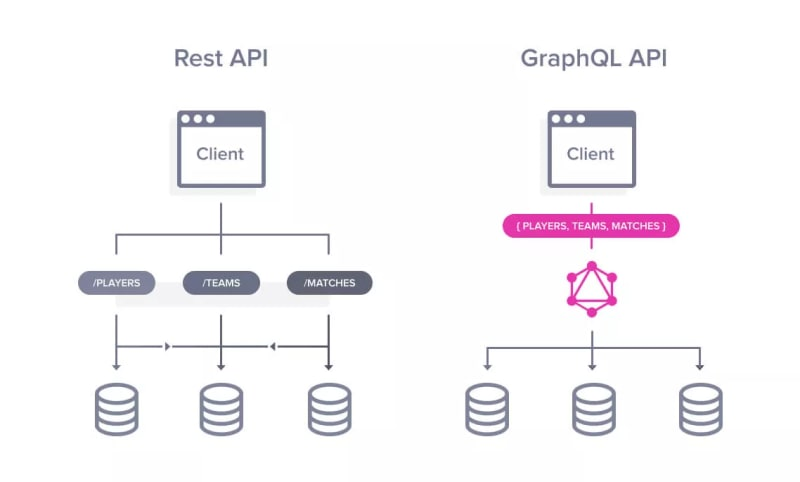
\includegraphics[width=0.8\textwidth]{Figures/graphql.jpg}
      \caption{GraphQL vs. REST Architecture}
      \label{fig:graphqlvsrestarchitecture}
\end{figure}
\begin{multicols}{2} % (json-rpc, xml-rpc, grpc) Webhooks API, Socket API Database API, Third-party API, Apache Thrift API, MsgPack API, SSE API, 
      \textbf{RPC API} : \acrshort{rpc} is a protocol return \acrshort{xml} or \acrshort{json} response. This protocol
      calls a method rather than a data resource, and remains one of the oldest and most stable protocols for
      \acrshort{api}s. While \acrshort{rest}ful \acrshort{api} returns a document, the response from a \acrshort{rpc}
      server is a confirmation that the function was triggered, or an error indicating  why it failed to run.

      \acrshort{rpc} is much faster than \acrshort{rest}, but the specifics depend on implementation. Unlike
      \acrshort{rest} or \acrshort{soap}, the message format varies. \acrshort{rpc} is tailored toward a client-server
      architecture and generally over a network.

      Components of a \acrshort{rpc} system:
      \begin{itemize}[label=$\star$]
            \item Client: the requesting device.
            \item Client stub: how the client will pack/unpack its materials.
            \item \acrshort{rpc} runtime: the messaging system (a courier between the client and server).
            \item Server stub: how the server will pack/unpack its materials.
            \item Server: the supplying device.
      \end{itemize}

      The popular frameworks of \acrshort{rpc}s are Apache Thrift, \acrshort{grpc}, and \acrshort{json}-\acrshort{rpc},
      and \acrshort{xml}-\acrshort{rpc}.

      \textit{gRPC}: developed by Google and released to public in 2015 to use, \acrshort{grpc} is an open-source
      \acrshort{rpc} architecture that can operate in numerous environments.

      The \acrshort{grpc} transport layer primarily relies on \acrshort{http}. The ability for developers to specify
      custom functions that allow for flexible inter-service communication is a significant feature of \acrshort{grpc}.
      This \acrshort{api} protocol also offers extra features such as timeouts, authentication, and flow control.

      In the \acrshort{grpc} protocol, data is transmitted in protocol buffers, a platform and language-agnostic mechanism
      that allows for data to be structured intuitively. This mechanism defines the service and then the data structures
      that the service will use. Compiling is taken care by protoc, the protocol buffer compiler.

      The output of this process is a comprehensive class containing the user's defined data types and basic set of methods
      in the chosen development language. Users can implement in-depth \acrshort{api} operations using this class.
\end{multicols}

\begin{lstlisting}[caption=gRPC Service For a Calculator In a Protobuf File]
      syntax = "proto3";

      package calculator;

      service Calculator {
            rpc Add(AddRequest) returns (AddResponse);
            rpc Subtract(SubtractRequest) returns (SubtractResponse);
      }

      message AddRequest {
            int32 a = 1;
            int32 b = 2;
      }

      message AddResponse {
            int32 result = 1;
      }

      message SubtractRequest {
            int32 a = 1;
            int32 b = 2;
      }

      message SubtractResponse {
            int32 result = 1;
      }
\end{lstlisting}

\begin{multicols}{2}
      \textit{Apache Thrift}: developed by Facebook, Thrift itself is a lightweight, language-agnostic software stack.
      This \acrshort{api} protocol supports \acrshort{http} transmission, along with binary transport formats. Thrift
      is capable of clean abstraction and implementations for data serialization and transport and application-level
      processing. Its primary objective is point-to-point \acrshort{rpc} implementation.

      Apache can support 28 programming languages, allowing programs written in any of these languages to communicate
      with each other and request remote services using \acrshort{api}s.
      \textbf{WebSocket}:
\end{multicols}

\begin{lstlisting}[language=JavaScript, caption=WebSocket's Example]
      // Client-side code
      const socket = new WebSocket('wss://example.com/socket'); // Replace with actual server's websocket URL
      
      // Event handler for when the connection is established
      socket.addEventListener("open", (event) => {
            console.log('Connected to the server');
            // Send data to the server
            socket.send('Hello, server!');
      });

      // Event handler for incoming messages from the server
      socket.addEventListener("message", (event) => {
            console.log(`Message from server: ${event.data}`);	
      });

      // Event handler for when the connection is closed
      socket.addEventListener("close", (event) => {
            console.log('Connection to the server closed');
      });

      // Event hander for handling errors
      socket.addEventListener("error", (event) => {
            console.error(`An error occurred: ${event.message}`);
      });
\end{lstlisting}

\begin{multicols}{2}
      \textbf{Socket}: is a software abstraction that allows programs running on different devices to
      communicate with each other over a network. It provides a standard interface for network
      communication, enabling data to be sent and received between applications running on separate
      computers. Sockets are commonly used in networking applications to establish connections and
      exchange data.
\end{multicols}

\begin{lstlisting}[language=Python, caption=TCP Server Example Using Sockets in Python]
      import socket

      # Create a TCP/IP socket
      server_socket = socket.socket(socket.AF_INET, socket.SOCK_STREAM)

      # Bind the socket to the address and port
      server_address = ('localhost', 8080)
      server_socket.bind(server_address)

      # Listen for incoming connections (max 5 clients in the queue)
      server_socket.listen(5)

      print('Server is listening on port 8080 for incoming connections....')

      while True:
            # Wait for a connection
            client_socket, client_address = server_socket.accept()

            try:
                  # Receive data from the client
                  data = client_socket.recv(1024)
                  print(f"Received data from {client_address}: {data.decode('utf-8')}")

                  # Send a response back to the client
                  response = 'Hello, client!'
                  client_socket.sendall(response.encode('utf-8'))

            finally:
                  # Clean up and close the connection
                  client_socket.close()
\end{lstlisting}

\begin{multicols}{2}
      \textbf{MsgPack}: is an open standard for compact binary data serialization, ideal for efficient data transfer.
      \acrshort{msgpack} supports a variety of data types, including integers, floating-point numbers, strings,
      arrays, maps (key-value pairs), and more. It is designed to be platform-agnostic, meaning that the data can be
      serialized in one programming language and deserialize it in another without compactibility issues.
\end{multicols}

\begin{lstlisting}[language=Python, caption=MsgPack Serialization and Deserialization in Python]
      import msgpack

      # Creating a Python dictionary to represent some data
      data = {
            'name': 'John Doe',
            'age': 30,
            'is_student': False,
            'hobbies': ['Reading', 'Gaming', 'Traveling'],
            'address': {
                  'street': 'Sesame Main Street',
                  'city': 'New York',
                  'zip': '10001'
            }
            "scores": [90, 85, 95, 100, 95, 88, 72]
      }

      # Serialize the data to a MsgPack binary format
      packed_data = msgpack.packb(data)

      # Deserialize the MsgPack binary data back to a Python object
      unpacked_data = msgpack.unpackb(packed_data)

      # Print the original data and the deserialized data
      print("Original data:", data)
      print("Unpacked data:", unpacked_data)
\end{lstlisting}

\begin{multicols}{2}
      With that being said, the \acrshort{qaas} app needs to manage and make connection different sort of \acrshort{api}s.
      Those \acrshort{api}s are the following:
      \begin{itemize}
            \item Resello: is used for \acrshort{qict} \acrshort{ms} subscriptions owned by Pax8. It is a cloud
                  marketplace that simplifies the way \acrshort{sme}s buy, sell, and manage cloud solutions through
                  automation. It provides a single platform to manage the entire cloud customer lifecycle, from
                  quote to cash to support, thus simplifying the process of buying, selling and managing cloud
                  solutions.
            \item SnelStart: is used for \acrshort{qict} automation of financial and accounting system software,
                  such as managing invoices, \acrshort{etc} for \acrshort{sme}s. It offers a range of products and
                  services to help businesses manage their finances, including accounting software, invoicing software,
                  and financial management tools.
            \item Bodyguard.io: is a \acrshort{cdr} tool used for security tab. It is a product from a Dutch company
                  that filters and scrutinizes downloads from web browsers to detect and prevent malicious files with
                  real-time download scanning capabilities.
            \item N-Central: is a product from N-Able and is used for monitoring clients' devices and ensuring the
                  overall security of their systems, \acrshort{it} infrastructure, and digital assets. It is a
                  \gls{RMM} platform designed to help \acrshort{msp} and \acrshort{it} professionals to
                  remotely monitor and manage their clients' devices and networks. It provides a comprehensive
                  set of tools and features for monitoring, managing, and securing clients' devices and networks,
                  including remote monitoring and management, patch management, antivirus, backup and disaster
                  recovery, and network topology mapping.
      \end{itemize}
      These different \acrshort{api}s will be discussed further in the next sub-question.
      \section{Research Sub-Question \#2}
      \subsection{What is API Monitoring?}
      \acrshort{api} monitoring is the process of gathering, visualizing, tracking, analyzing, and alerting on the
      performance, availability, and the \acrshort{api} telemetry data to ensure that \acrshort{api} requests are
      handled as expected.
      \subsection{How Does API Monitoring Work?}
      \acrshort{api} monitoring automatically checks \acrshort{api} performance and availability at regular intervals,
      to ensure that the \acrshort{api} runs appropriately. This can be done in a few different ways, depending on the
      type of the \acrshort{api} being monitored~\ref{chap:typesofapis}.

      For example, let's take Postman, a popular free \acrshort{api} monitoring tools that allows developers to easily
      monitor, analyze, and debug their \acrshort{api}s. In this example, the system might look for common errors, such
      as 500-level responses or timeouts, when making requests to the \acrshort{api}. It also checks for latency issues
      or sudden spikes in traffic that could indicate potential system problems. In addition, this monitoring system can
      be configured to track specific metrics such as total requests, response times, and other \acrshort{kpi}s over time.
      This will then provide real-time insights into \acrshort{api} performance and offers a range of features such as
      automated alerts, detailed analytics, and comprehensive reporting capabilities. Features that an \acrshort{api}
      monitoring might have are listed in the following (\cite{postmanapimonitoring}):
      \begin{itemize}
            \item \textbf{Endpoint Surveillance}: it begins by closely tracking the various endpoints of an \acrshort{api}
                  system. These endpoints represent specific functionalities or resources that the \acrshort{api} provides.
            \item \textbf{Request-Response Analysis}: monitoring tools can simulate \acrshort{api} requests by sending
                  predefined inputs and parameters to specific endpoints, then analyzing the responses for relevant factors
                  such as response time or data accuracy.
            \item \textbf{Performance Metrics Measurement}: \acrshort{kpi}s, such as response time, latency, and error rates,
                  are measured and tracked over time. This metrics offers insights into the overall health and efficiency of
                  an \acrshort{api}.
            \item \textbf{Error Detection and Logging}: actively identifying and log any errors or anomalies in \acrshort{api}
                  resources with an \acrshort{api} monitoring program. This includes capturing \acrshort{http} error codes,
                  unexpected data/file formats, and alerting of any deviations from expected behaviour.
            \item \textbf{Security Checks}: \acrshort{api} monitoring assess \acrshort{api} transactions for unauthorized
                  access attempts, potential vulnerabilities, and adherence to security protocols.
            \item \textbf{Alerting and Notification System}: automated alerting systems can be configured with high levels of
                  customization to notify relevant stakeholders when specific \acrshort{api} performance thresholds are breached
                  or exceeded or when abnormal behaviour is detected.
            \item \textbf{Usage Analysis Gathering}: collect usage analytics for insights into how a given \acrshort{api} is
                  being used. This data helps software organizations plan for scalability, optimize resource allocation, and
                  understand user behaviour.
            \item \textbf{Logging for Auditing}: detailed logs of \acrshort{api} interactions are maintained for auditing
                  purposes. These \acrshort{api} logs are valuable resources for post-incident analysis and tracking historical
                  performance and behavioural trends.
            \item \textbf{Continuous Monitoring}: the tool is a constantly ongoing, real-time process that ensures that
                  issues of any scope are identified and addressed promptly.
      \end{itemize}
      With those functionalities in mind, \acrshort{api} monitoring tools can then automatically check \acrshort{api}
      performance and availability at specified intervals of time to ensure that the monitored \acrshort{api}s run
      appropriately. The specific timing of those intervals is unique to each \acrshort{api} product.
      \section{Research Sub-Question \#3}
      \subsection{SentinelOne} % vs CrowdStrike with Carbanak and FIN7 methodology, Huntresss, datto rmm
      SentinelOne is a cybersecurity platform that provides endpoint protection, detection, and response capabilities to
      help organizations defend against advanced cyber threats. It leverages \acrlong{ai} and machine learning to analyze
      and respond to security threats in real-time, providing organizations with comprehensive protection against malware,
      ransomware, and other cyber threats. It also provides visibility into clients' \acrshort{it} systems and infrastructure,
      enabling organizations to gain insights into potential security risks and vulnerabilities and take proactive measures
      to address them.
      \subsection{SentinelOne Console}
      \subsection{Ranger}
      Ranger is one of the SentinelOne product that provides a way of detecting other devices (computers and
      \acrshort{iot} devices) that are on the client's computer network. If a malicious attacker comes in and plugs his device
      into the network, all the other SentinelOne agents are going to read the network traffic, determine and classify whether
      this is a new device, or a rogue device. As long as a device has Ranger on that network subnet, SentinelOne can gather and
      detect technical information regarding the device. On a network, before a machine is connected and talks to other devices
      and gateways, it is going to do a broadcast and gives up information about itself. This is called an \acrshort{arp} request.
      Ranger is going to read that \acrshort{arp} request and determine

      \subsection{Sentinels}
      Sentinels are the end-points,
      \subsection{SentinelOne Agent}
      An Agent is a software program, deployed to each endpoint, including desktop, laptop, server or virtual environment,
      and runs autonomously on each device, without reliance on internet connection.
      \subsection{Vigilance}
      It is a \acrshort{mdr} service - providing threat monitoring, hunting, and response, to its existing customers. It
      provides a 24/7 \acrshort{soc} with expert analysts and researchers to give customers near real-time threat monitoring,
      in-console threat annotations, and response to threats and suspicious events.
      \subsection{Incidents}

      \section{Research Sub-Question \#4}
\end{multicols}